\documentclass[times, utf8, zavrsni]{fer}
\usepackage{booktabs}
\usepackage{listingsutf8}
\usepackage[titletoc]{appendix}
\usepackage[page]{appendix}
\renewcommand{\figurename}{Slika}
\renewcommand{\contentsname}{Sadržaj}
\renewcommand{\appendixname}{Dodatak}
\begin{document}

% TODO: Navedite broj rada.
\thesisnumber{1337}

% TODO: Navedite naslov rada.
\title{Obrada podataka tehnologijom Apache Spark}

% TODO: Navedite vaše ime i prezime.
\author{Martin Matak}

\maketitle

% Ispis stranice s napomenom o umetanju izvornika rada. Uklonite naredbu \izvornik ako želite izbaciti tu stranicu.
\izvornik{Na ovoj stranici se nalazi izvornik.}

% Dodavanje zahvale ili prazne stranice. Ako ne želite dodati zahvalu, naredbu ostavite radi prazne stranice.
\zahvala{Zahvala - TODO \ldots :)}

\tableofcontents

\chapter{Uvod}
\section{Motivacija}
%Literatura: http://mob.hr/samsung-galaxy-s4-skrivene-mogucnosti-senzori-i-octa-5-benchmark/
Pametni mobilni uređaji postaju neizostavan dodatak svakog modernog čovjeka.\\
Većina pametnih mobilnih uređaja u sebi sadrži sljedeće senzore:
\begin{description}
	\item[akcelerometar] - elektromehanička komponenta koja mjeri sile ubrzanja;
	\item[barometar] - mehanički senzor za mjerenje atmosferskog pritiska (na trenutnoj lokaciji uređaja);
	\item[senzor svjetlosti] - mjeri intenzitet, tj. jačinu svjetlosti i uglavnom se nalazi s prednje strane uređaja, iznad ekrana;
	\item[senzor blizine] - u stanju prepoznati situacije kada mu neki objekt stoji u blizini - ovo omogućava automatske pozive prilikom primicanja telefona licu uz zaključavanje telefona da bi onemogućili slučajno prekidanje poziva uhom ili slično;
	\item[senzor gestikulacije] - prepoznaje kretnje ruke tako što detektira infracrvene zrake koje se reflektiraju - omogućuje nam djelomično upravljanje telefonom bez doticanja ekrana;
	\item[žiroskop] - uređaj koji se koristi za navigaciju i merenje kutne brzine;
	\item[geomagnetski senzor] - mjeri okolno geomagnetsko polje za sve tri fizičke osi i u biti služi kao kompas na mobilnim uređajima i 
	\item[\emph{Hall Sensor}] - magnetski senzor zadužen za prepoznavanje je li  maska telefona zatvorena ili otvorena.
\end{description}
Pretpostavimo da je mobilni uređaj spojen na internet i da svakih nekoliko sekundi pošalje vrijednost koju u tom trenutku mjeri pojedini senzor. U samo jednom danu može se skupiti dosta podataka. A što kada to ne bi radili za jedan uređaj nego za sve izdane uređaje nekog modela? Količina podataka bi jako brzo narasla.

Kako količina podataka postaje sve veća, dolazimo do pojma \emph{Velika količina podataka} \engl{Big Data}. U današnje vrijeme imamo više podataka u digitalnom obliku nego što smo ikada imali. Jedan od zanimljivijih izazova je kako ih efektivno obraditi i zaključiti nešto iz toga. Kako od te velike količine podataka doći do nekih pametnih zaključaka iz kojih ćemo nešto novo naučiti.

\emph{Apache Spark} je otvorena \engl{open source} tehnologija koja omogućava pisanje programa za obradu podataka u tri programskih jezika: \emph{Java}, \emph{Python} i  \emph{Scala}; a nudi i mogućnost interaktivnog rada. \\
U okviru ovog rada biti će proučene mogućnosti ove tehnologije, razrađeno nekoliko konkretnih primjera obrade podataka te ostvarena programska rješenja koja obavljaju tu obradu koristeći \emph{Apache Spark}.

Svi primjeri će biti napisani u programskom jeziku \emph{Java}.

\section{Instalacija i izvorni kodovi}
\subsection{Instalacija}
\emph{Apache Spark} je pisan u programskom jeziku \emph{Scala} i izvršava se na \emph{Javinom virtualnom stroju} \engl{Java Virtual Machine} (JVM). Instalacija na osobno računalo je prilično jednostavna, a u ovdje će biti prikazana instalacija na operacijskom sustavu \emph{Ubuntu 15.10}. \\
Za početak je potrebno imati instaliranu Javu, a je li Java instalirana na računalu se može provjeriti tako što se u naredbenom retku unese sljedeća naredba:\\
\texttt{java -version}. Kao rezultat bi trebali dobiti trenutno instaliranu verziju Jave. Ukoliko Java nije instalirana, potrebno ju je najprije instalirati. Taj dio neće biti objašnjen ovdje.

Jednom kada imamo instaliranu Javu, sve što treba napraviti je otići na službene stranice: \url{https://spark.apache.org/downloads.html}, odabrati najnoviju verziju (Za vrijeme pisanja ovog rada to je verzija \emph{1.6.1 (Mar 09 2016}), izabrati odgovarajući paket te pokrenuti dohvaćanje odgovarajuće \emph{.tgz} arhive. Najjednostavnije je odabrati neki \emph{pre-built} paket, primjerice \emph{Pre-built for Hadoop 2.6 and later} te će daljnji koraci instalacije biti napisani pod pretpostavkom da je korisnik dohvatio tu verziiju paketa. Ukoliko korisnik želi, moguće je instalirati i \emph{Source code} varijantu paketa, ali taj postupak instalacije ovdje nije opisan. 

Nakon što smo dohvatili odgovarajuću arhivu, potrebno ju je raspakirati.\\ Raspakiranje arhive moguće je napraviti preko naredbe:
\begin{lstlisting}[language=bash]
$ tar -xvf spark-1.6.1-bin-hadoop2.6.tgz
\end{lstlisting}
Nakon toga, dobra je praksa premjestiti instalaciju u neki prikladniji direktorij. Tako nešto može se napraviti na sljedeći način:
\begin{lstlisting}[language=bash]
$ mv Downloads/spark-1.6.1-bin-hadoop2.6 faks/spark/
\end{lstlisting}
Službeno, sada je instalacija gotova. Idemo u sljedećem odlomku malo detaljnije pogledati što smo to zapravo dobili instalacijom. Koje datoteke se sada nalaze na našem računalu, a nije ih bilo ranije. Također, biti će objašnjena i uloga nekih datoteka i direktorija.

\subsection{Izvorni kodovi}
Ako izlistamo što nam se trenutno nalazi u novonastalom direktoriju, dobiti ćemo sljedeći ispis:
\begin{lstlisting}[language=bash]
mmatak@martins-beast:~/faks/spark$ ls -l
total 1408
drwxr-xr-x 2 mmatak mmatak    4096 Feb 27 06:02 bin
-rw-r--r-- 1 mmatak mmatak 1343562 Feb 27 06:02 CHANGES.txt
drwxr-xr-x 2 mmatak mmatak    4096 Feb 27 06:02 conf
drwxr-xr-x 3 mmatak mmatak    4096 Feb 27 06:02 data
drwxr-xr-x 3 mmatak mmatak    4096 Feb 27 06:02 ec2
drwxr-xr-x 3 mmatak mmatak    4096 Feb 27 06:02 examples
drwxr-xr-x 2 mmatak mmatak    4096 Feb 27 06:02 lib
-rw-r--r-- 1 mmatak mmatak   17352 Feb 27 06:02 LICENSE
drwxr-xr-x 2 mmatak mmatak    4096 Feb 27 06:02 licenses
-rw-r--r-- 1 mmatak mmatak   23529 Feb 27 06:02 NOTICE
drwxr-xr-x 6 mmatak mmatak    4096 Feb 27 06:02 python
drwxr-xr-x 3 mmatak mmatak    4096 Feb 27 06:02 R
-rw-r--r-- 1 mmatak mmatak    3359 Feb 27 06:02 README.md
-rw-r--r-- 1 mmatak mmatak     120 Feb 27 06:02 RELEASE
drwxr-xr-x 2 mmatak mmatak    4096 Feb 27 06:02 sbin
\end{lstlisting}

\begin{description}
\item[\emph{README.md} ]Sadrži kratke instrukcije za upoznavanje sa Spark-om.
\item[\emph{bin} ]Sadrži izvršive datoteke koje se koriste za interaktivni rad sa Spark-om.\\Zanimljivo je spomenuti da postoji interaktivna ljuska \emph{Spark shell} za programske jezike \emph{Python} i \emph{Scala}. Datoteke u ovom direktorij služe upravo za to. Budući da je ovaj rad ograničen isključivo na programski jezik \emph{Java}, ovaj dio neće biti detaljnije obrađen.
\item[\emph{core, streaming, python, ...} ]Sadrži glavne komponente projekta \emph{Apache Spark} 
\item[\emph{examples} ]Sastoji se od nekoliko jednostavnih primjera koje pomažu korisniku da se uhoda i što bezbolnije nauči koristiti odgovarajući API.
\end{description}

Kako bi bili sigurni da je instalacija uspješna, potrebno je pozicionirati se u \emph{bin} direktorij te u terminalu upisati \texttt{./spark-shell}. Ispis bi trebao biti sličan ovome:\\
\begin{lstlisting}[language=bash]
mmatak@martins-beast:~/faks/spark/bin$ ./spark-shell
Welcome to
      ____              __
     / __/__  ___ _____/ /__
    _\ \/ _ \/ _ `/ __/  '_/
   /___/ .__/\_,_/_/ /_/\_\   version 1.6.1
      /_/

Using Scala version 2.10.5 (OpenJDK 64-Bit Server VM, Java 1.8.0_91)
Type in expressions to have them evaluated.
Type :help for more information.
scala>
\end{lstlisting}


Ukoliko se prikaže greška vezana uz \emph{sqlContext}, to je OK. U ovom trenutku to nije važno. Važno je napomenuti da su u gornjem ispisu (radi ljepšeg formata ovog rada) izbrisana upozorenja \engl{warnings} koja su normalna i očekivana.

\newpage
\section{Osnovni gradivni elementi}
Osnovna programska apstrakcija s kojom \emph{Apache Spark} radi naziva se \emph{resilient distributed dataset} (RDD). RDD-ovi predstavljaju kolekcije podataka koje se nalaze na računalima (jednom ili više njih) i moguće ih je paralelno obrađivati. \emph{Apache Spark} nudi bogati API za rad s RDD-ovima.

\emph{Apache Spark} se sastoji od nekoliko ključnih elemenata koji će ovdje biti samo nabrojani i opisani rečenicom ili dvije, a u kasnijim poglavljima će biti detaljnije objašnjeni. Slika koja predstavlja osnovne elemente je sljedeća: 
%preuzeto s http://spark.apache.org/images/spark-stack.png
\begin{figure}[htb]
\centering
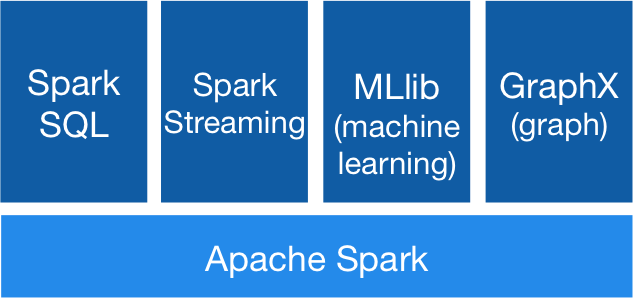
\includegraphics[width=10cm]{img/spark-stack.png}
\caption{Osnovni elementi tehnologije \emph{Apache Spark}.}
\label{fig:spark-stack}
\end{figure}

Na slici su prikazana četiri osnovna elementa koja čine osnovu tehnologije \emph{Apache Spark}, a to su: 
\begin{description}
\item[\emph{Spark SQL}] - omogućuje rad s bilo kakvim strukturiranim podatcima, primjerice JSON. Nudi mogućnost izvršavanja SQL-a nad RDD-ovima;
\item[\emph{Spark Streaming}] - komponenta zadužena za rad s tokovima podataka;
\item[\emph{MLib}] - koristi se za postupak strojnog učenja i 
\item[\emph{GraphX}] - biblioteka za obradu grafova (npr. graf prijatelja na društvenoj mreži).
\end{description}

\section{Kratki pregled}
U ovom poglavlju je bila ideja da čitatelj dobije motivaciju i želju za upoznavanjem s tehnologijom \emph{Apache Spark}. Detaljno je opisan postupak instalacije koji bi čitatelju trebao biti sasvim dovoljan za samostalnu instalaciju. Također, dan je pregled nekih najosnovnijih datoteka i direktorija koje dolaze s instalacijom. Zainteresiranog čitatelja se ohrabruje da samostalno prouči kako se koristi \emph{Spark shell}. Na kraju, nabrojani su osnovni elementi koji čine jezgru tehnologije \emph{Apache Spark} i uveden je pojam osnovne programske apstrakcije koja se koristi u ovoj tehnologiji, a to je \emph{resilient distributed dataset} (RDD).

\chapter{Prvi programi}
\section{Postavljanje temelja}
\subsection{Osnovni elementi aplikacije}
Općenito govoreći, svaka Spark aplikacija sastoji se od nekoliko komponenata. Prva komponenta koju ćemo spomenuti je program koji se izvršava - onaj čija je \texttt{main} metoda pokrenuta, odnosno onaj koji pokreće obradu podataka. Taj program se naziva \emph{driver}. On s podatcima priča kroz "tunel" između sebe i Sparka odnosno kroz \emph{SparkContext}. Budući da je \emph{Apache Spark} namijenjen za paralelnu obradu podataka, idemo se odmah upoznati i s još dvije komponente. Pojedino računalo u \emph{grozdu} \engl{cluster} ćemo nazvati \emph{radnim čvorom} \engl{worker node}, a proces koji se izvršava na pojedinom računalu nazvati ćemo \emph{radnik} \engl{executor}. Dozvoljeno je da \emph{radnici} međusobno komuniciraju. U cijeloj priči može, a i ne mora eksplicitno biti uključen \emph{upravitelj grozdom} \engl{cluster manager}.

%Izvor slike: http://spark.apache.org/docs/latest/cluster-overview.html

\begin{figure}[htb]
\centering
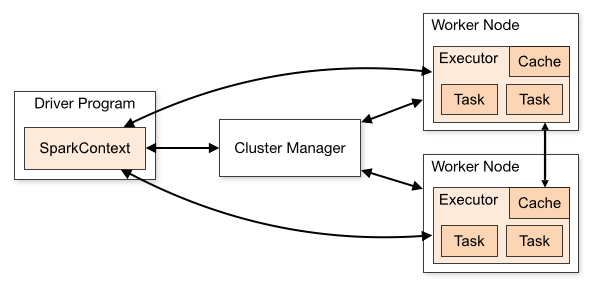
\includegraphics[width=10cm]{img/cluster-overview.png}
\caption{Prikaz elemenata aplikacije.}
\label{fig:cluster-overview}
\end{figure}
\subsection{Programiranje u Javi}
Kako bi mogli pisati Spark programe u programskom jeziku \emph{Java}, potrebno je povezati svoju aplikaciju s \texttt{spark-core} artifaktom s Mavena. Za postavljanje i instalaciju Mavena konzultirati \url{https://maven.apache.org/install.html} i knjigu (Programiranje u Javi, Čupić). Za vrijeme pisanja ovog rada, najnovija verzija Sparka je 1.6.1, a odgovarajuće Maven koordinate su:
\begin{lstlisting}[language=bash]
groupId = org.apache.spark
artifactId = spark-core_2.10
version = 1.6.1
\end{lstlisting}
Odgovarajuća \texttt{pom.xml} datoteka nalazi se u dodatku \ref{ch:datotekapomXML}.

Jednom kada smo namjestili \texttt{pom.xml} datoteku i povezali se s \texttt{spark-core}, sve što trebamo još napraviti je inicijalizirati \emph{SparkContext} i napisati prvu aplikaciju. U nastavku je jednostavna aplikacija koja jedino što radi je broji koliko riječi ima u tekstualnoj datoteci.
\section{Programiranje s RDD-ovima}


\chapter{Zaključak}
Zaključak.

\bibliography{literatura}
\bibliographystyle{fer}

\newpage
% Dodatak nije obavezan
\begin{appendices}
\chapter{Postavljanje datoteke pom.xml}
\label{ch:datotekapomXML}
Datoteka koja je potrebna kako bi Maven ispravno dohvatio artifakt \texttt{spark-core} bi trebala izgledati slično kao što je dano u nastavku. Za ispravno funkcioniranje, trebala bi se zvati \texttt{pom.xml} i nalaziti se direktno u direktoriju \texttt{src}.
\begin{lstlisting}[language=XML]
<project>
  <modelVersion>4.0.0</modelVersion>
  <groupId>hr.fer.zemris</groupId>
  <artifactId>Prva Spark aplikacija</artifactId>
  <packaging>jar</packaging>
  <version>1</version>
  <name>Prva Spark aplikacija</name>	
  <url>http://maven.apache.org</url>
  <dependencies>
    <dependency>
	<groupId>org.apache.spark</groupId>
	<artifactId>spark-core_2.10</artifactId>
	<version>1.6.1</version>
    </dependency>
  </dependencies>
</project>
\end{lstlisting}
\end{appendices}

\begin{sazetak}
Sažetak na hrvatskom jeziku.

\kljucnerijeci{Ključne riječi, odvojene zarezima.}
\end{sazetak}

% TODO: Navedite naslov na engleskom jeziku.
\engtitle{Title}
\begin{abstract}
Abstract.

\keywords{Keywords.}
\end{abstract}

\end{document}
